\subsection{Kanter}\label{subsec:kant}
Hvis et billede beskues i 3D, kan en kant illustreres i 1D, ved et snit af et billede vinkelret på overfladen. En kant er et stort intensitetsskift, som illustreret figur \ref{fig:kant}.
\noindent
\begin{figure}[H]
    \centering
    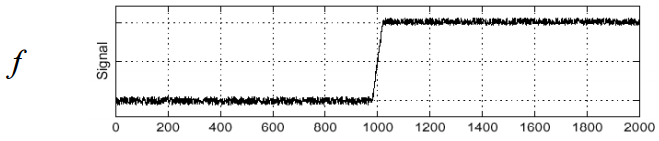
\includegraphics[width=0.55\textwidth]{fig/7.png}
     \vspace{-1em}
    \begin{center}        
     \caption{\textcolor{gray}{\footnotesize \textit{
     En 1-dimensional fortolkning af intensiteten i et billede. De små udsving indikere støj, den store kurve repræsenter et skift i intensiteten og derved en kant i et billedet.}}}
    \label{fig:kant}
     \end{center}
       \vspace{-2.5em}
  \end{figure}
\noindent
En differentiering af funktionen fra figur \ref{fig:kant} vil fremhæve dens udsving og derved angive hvor der forekommer kanter. 
\\
\\
Et billede i 2D er ikke en kontinuerlig funktion, men består af diskrete værdier i form af pixelværdier.
Differentiering af billeder kan approsikmeres ved følgende ligning:
\begin{equation}
\dfrac{df(x)}{dx}=\dfrac{f(x+1)-f(x-1)}{2}
\label{diff}
\end{equation}
Foldning af $I$ af størrelse $(M \times N)$, med en kerne $K$ der har størrelse $(m \times n)$, hvor $M > k, N > n$:
\begin{equation}
O(i,j) = \sum\limits_{x=1}^m \sum\limits_{y=1}^n I(i+k-1,l-1)K(k,l)
\label{foldning}
\end{equation}
Ligning \eqref{foldning} sker for alle $i,j \in I$. \\
Et billede kan differentieres, som ligning \eqref{foldning}, ved brug af foldning. Først defineres en kerne til horizontal differentiering $K$, som: $K = [\frac{1}{2}, 0, \frac{1}{2}]$. Kernen foldes med billedet $I$: $I \ast K $, hvor $\ast$ udgør foldningsoperatoren.
\\
\\
I grænsetilfælde, skal en kerne foldes med et billede, hvor afstanden til kanten af billedet, er skarpt mindre, end størrelsen af kernen - dvs. der iflg ligning \eqref{foldning} ganges med et område, hvor $i < 0, j < 0$. Her gælder $I(i < 0, j < 0) = 0$. Eg. $O(1,1)$, med en kerne der har størrelse $M > m > 1$, $N > n > 1$, vil værdien af $I(i+k-1 < 0, l-1 <0) = 0$  \\
\\
Problemet ved differentiering, visualiseret i figur \ref{fig:kant}, er at støj i billedet (de små udsving) også vil blive fremhævet, hvilket kan resultere i fejlagtige detektioner af kanter. For at fjerne støjen kan billedet foldes et kan Gaussisk filter, hvilket er en diskret approksimering til den Gaussiske funktion. Foldning af et billede med et Gaussisk filter vil resultere i en "flydende" overgang mellem pixel værdierne og derfor glatte billedet. Den Gaussiske funktion i 2-D, hvor $ \sigma $ er standardafvigelsen af den Gaussiske fordelingen, er defineret som:
\begin{equation}
G(x,y,\sigma) = \frac{1}{2 \pi \sigma ^{2}} e^{- \frac{x^{2} + y^{2}}{2 \sigma ^{2}}}
\label{2dgaussian}
\end{equation} 
For at undgå først at glatte billedet ved at folde med et Gaussfilter, og derefter folde med et differentieringsfilter, udnyttes at foldning er en associativ operation:
\begin{equation}
\dfrac{\partial}{\partial x}(G \ast f) = (\dfrac{\partial}{\partial x}G) \ast f
\end{equation}
Foldes et 1 dimensionelt gaussfilter med signalet fra figur \ref{fig:kant}, vil det resultere i et bakkeformet signal, hvor bakken indikere en kant. For en mere lokaliserbar kant, kan den dobbelt afledte tages, som set i figur \ref{fig:deriv}.
\begin{figure}[H]
    \centering
    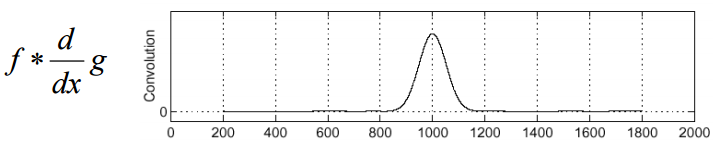
\includegraphics[width=0.55\textwidth]{fig/8.png}
    \vspace{-1em}   
    \begin{center}
    \caption{\textcolor{gray}{\footnotesize \textit{
     Resultatet af at folde et dobbelt differentieret Gaussisk filter med funktionen}}}
    \label{fig:deriv}
     \end{center}
    \vspace{-2.5em}  
  \end{figure}
\noindent
Kanten kan nu lokaliseres, ved at identificere funktionens nul-krydsning (zero-crossing).